\documentclass{beamer}
\usetheme{Madrid}
\setbeamertemplate{navigation symbols}{}

\usepackage{amsmath}
\usepackage{graphicx}
\usepackage{multicol}
\usepackage{multirow}
\usepackage{array}

\usepackage{tikz}
\usetikzlibrary{shapes.geometric, shapes.misc, arrows}
\usetikzlibrary{calc}
\usetikzlibrary{positioning}

\usepackage{multirow}  % use tables with columns stretching over multiple rows
\usepackage{booktabs}

\usepackage{pgfplots}
\pgfplotsset{compat=1.18}

\pgfplotsset{
  report_style/.style={
    legend style={draw=none, font=\small},
    legend cell align=left,
    legend pos=north east,
    ylabel style={align=center, font=\bfseries\boldmath},
    xlabel style={align=center, font=\bfseries\boldmath},
    x tick label style={font=\bfseries\boldmath},
    y tick label style={font=\bfseries\boldmath},
    scaled ticks=false,
    every axis plot/.append style={thick},
  },
}

\usepackage[justification=centering]{caption}
\usepackage{subcaption}

\usepackage{xurl}

% default path to images and other assets
\graphicspath{{../assets/}}

% disable wrapping
\tolerance=1
\emergencystretch=\maxdimen
\hyphenpenalty=10000
\hbadness=10000

% number figure caption
\setbeamertemplate{caption}[numbered]

% display bib label in references
\setbeamertemplate{bibliography item}{\insertbiblabel}
\setbeamertemplate{bibliography entry title}{}
\setbeamertemplate{bibliography entry location}{}
\setbeamertemplate{bibliography entry note}{}

% \newcommand{\fall}[1]{\quad \textcolor{red}{#1}}
\newcommand{\src}[1]{#1^{src}}
\newcommand{\tgt}[1]{#1^{tgt}}
\newcommand{\floor}[1]{\left\lfloor #1 \right\rfloor}
\newcommand{\ceil}[1]{\left\lceil #1 \right\rceil}
\newcommand*\quot[2]{{^{\textstyle #1}\big/_{\textstyle #2}}}
\DeclareMathOperator*{\argmax}{arg\,max}

% Metadata
% ------------------------
\title[XLNER]{Formalization of natural language processing tasks as optimization problems}
\subtitle{Master thesis}

\author[Oleh Shkalikov]{Oleh Shkalikov\texorpdfstring{ (5102818)
    \\[0.7em]{\small Supervisor: Jannik Irmai}
\\{\small Reviewers: Prof. Dr. Bjoern Andres, Prof. Dr. Simon Razniewski}}{}}

\institute[TU Dresden]{TU Dresden}

\date{January 24, 2025}

\begin{document}

\frame{\titlepage}

% \begin{frame}
%   \frametitle{Table of contents}
%   \tableofcontents
% \end{frame}

\section{Introduction}

\begin{frame}
  \frametitle{Named Entity Recognition}

  \begin{figure}[ht]
    \centering
    \begin{tikzpicture}[node distance=0.1,
        every node/.style={text centered,
          text height=2ex,
          text depth=.25ex,
        },
        loc/.style={fill=orange!30, rounded rectangle, label={[anchor=center,font=\tiny\bfseries\sffamily]above:####1-LOC}},
        per/.style={fill=green!30, rounded rectangle, label={[anchor=center,font=\tiny\bfseries\sffamily]above:####1-PER}},
        O/.style={rounded rectangle, label={[anchor=center,font=\tiny\bfseries\sffamily]above:O}}
      ]

      \node[per={B}, rounded rectangle east arc=none](Mark){Mark};
      \node[per={I}, rounded rectangle west arc=none, right=of Mark](Twain){Twain};
      \node[O, right=of Twain](was){was};
      \node[O, right=of was](born){born};
      \node[O, right=of born](in){in};
      \node[loc={B}, right=of in]{Florida};
    \end{tikzpicture}
    \caption{Example of NER labeling in IOB2 format}
    \label{fig:ner}
  \end{figure}
\end{frame}

\begin{frame}
  \frametitle{Issues of multilingual NER}
\end{frame}

\section{Related works}

\begin{frame}
  \frametitle{Classification of approaches to XLNER}

  \begin{figure}
    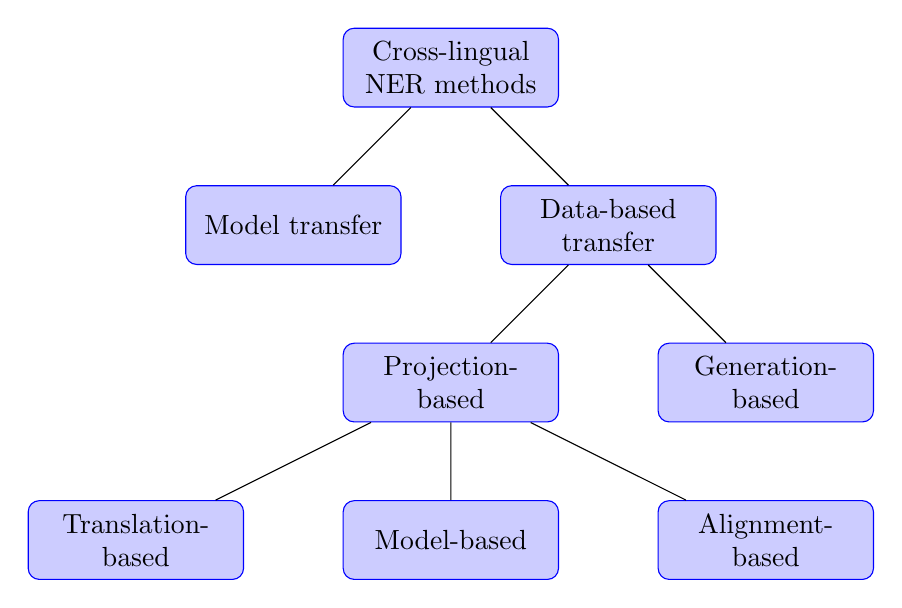
\begin{tikzpicture}[nodes={rectangle, rounded corners,
          minimum width=2cm, text width=2.5cm, minimum height=1cm,
        text centered, draw=blue, fill=blue!20},
        sibling distance=4cm, level distance=2cm,
      ]
      \node {Cross-lingual NER methods}
      child {node(a){Model transfer} edge from parent}
      child {node(b){Data-based transfer}
        child {node(d){Projection-based}
          child {node(e){Translation-based}}
          child {node(e){Model-based}}
          child {node(e){Alignment-based}}
        }
        child {node(c){Generation-based} edge from parent}
      };
    \end{tikzpicture}
  \end{figure}
\end{frame}

\begin{frame}
  \frametitle{Model transfer}
\end{frame}

\begin{frame}
  \frametitle{Projection-based pipeline}

  \begin{figure}
    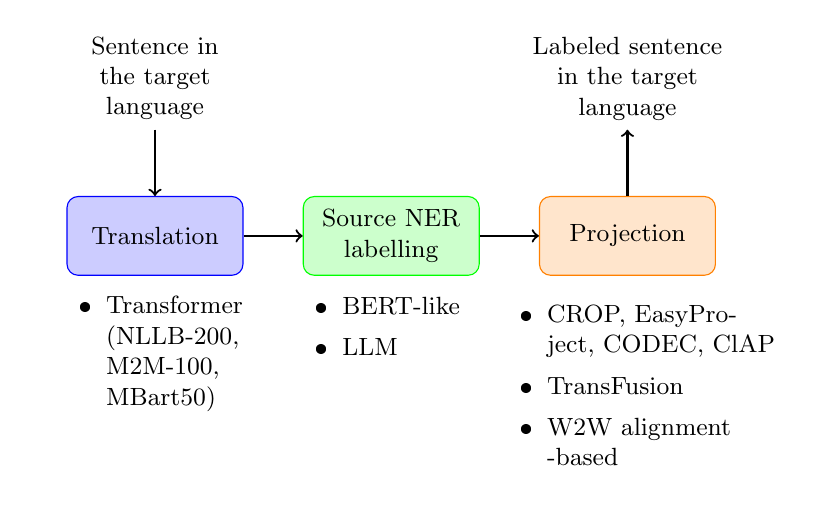
\begin{tikzpicture}[
        nodes={text width=2cm, minimum height=1cm,
        text centered, font = {\small}},
        step_style/.style={rectangle, rounded corners},
        text_style/.style={text width=3cm},
      node distance=3cm]

      % \draw[dashed] (1.5, 0) -- (1.5, 7);

      \node (orig_text) at (0,0) {Sentence in the target language};
      \node[step_style, draw=blue, fill=blue!20, below of=orig_text, yshift=1cm] (fwd_trans) {Translation};
      \node[step_style, draw=green, fill=green!20, right of=fwd_trans] (source_ner) {Source NER labelling};
      \node[step_style, draw=orange, fill=orange!20, right of=source_ner] (proj) {Projection};
      \node[above of=proj, yshift=-1cm, text width=2.5cm] (labeled_orig) {Labeled sentence in the target language};

      \node[text_style, below of=fwd_trans, yshift=1.5cm] {\vbox {
          {
            \begin{itemize}
              \item Transformer (NLLB-200, M2M-100, MBart50)
            \end{itemize}}}};
      \node[text_style, below of=source_ner, yshift=1.85cm] {\vbox {
          {
            \begin{itemize}
              \item BERT-like
              \item LLM
            \end{itemize}}}};
      \node[text_style, below of=proj, yshift=1.1cm, text width=3.8cm] {\vbox {
          {
            \begin{itemize}
              \item CROP, EasyProject, CODEC, ClAP
              \item TransFusion
              \item W2W alignment -based
            \end{itemize}}}};

      \draw[->, thick] (orig_text) -- (fwd_trans);
      \draw[->, thick] (fwd_trans) -- (source_ner);
      \draw[->, thick] (source_ner) -- (proj);
      \draw[->, thick] (proj) -- (labeled_orig);
    \end{tikzpicture}
    \caption{General scheme of projection-based pipelines}
  \end{figure}
\end{frame}

\begin{frame}
  \frametitle{Translation-based projection}
\end{frame}

\begin{frame}
  \frametitle{Model-based projection}
\end{frame}

\begin{frame}
  \frametitle{Word-to-word alignment-based projection}
\end{frame}

\section{Methodology}

\begin{frame}
  \frametitle{Requirements to the formalization}
\end{frame}

\begin{frame}
  \frametitle{Projection ILP problem}

  \begin{align*}
    & \max\limits_x \sum\limits_{(\src{p}, \tgt{p}) \in S \times T} c_{\src{p}, \tgt{p}} x_{\src{p}, \tgt{p}} \\
    & \text{subject to}                                                                                                                      \\
    & \sum\limits_{\tgt{p} \in T} x_{\src{p}, \tgt{p}} \lessgtr n_{proj}
    \; \qquad \forall \src{p} \in S \\
    & x_{\src{p_1}, \tgt{p_1}} + x_{\src{p_2}, \tgt{p_2}} \leq 1
    \qquad \forall (\src{p_1}, \src{p_2}, \tgt{p_1}, \tgt{p_2}) \in \hat{\Pi}(S, T) \\
    & x_{\src{p}, \tgt{p}} \in \{ 0, 1 \}
    \; \;\qquad \qquad \forall (\src{p}, \tgt{p}) \in S \times T \notag
  \end{align*}
  where
  \begin{align*}
    \hat{\Pi}(S, T) = \Big\{ (\src{p_1}, \src{p_2}, \tgt{p_1}, \tgt{p_2}) \Big| \src{p_1}, \src{p_2} \in S, \tgt{p_1}, \tgt{p_2} \in T, \\
      \tgt{p_1} \cap \tgt{p_2} \neq \emptyset,
    (\src{p_1} \neq \src{p_2}) \lor (\tgt{p_1} \neq \tgt{p_2}) \Big\}
  \end{align*}
\end{frame}

\begin{frame}
  \frametitle{Reduction of the non-overlapping constraints}

  \begin{block}{Theorem}

    The set of non-overlapping constraints is satisfied if and only if
    the following sets of reduced constraints are satisfied:
    \begin{align*}
      & \sum\limits_{\src{p} \in S} (x_{\src{p}, \tgt{p_1}} + x_{\src{p}, \tgt{p_2}}) \leq 1
      \qquad \forall (\tgt{p_1}, \tgt{p_2}) \in \Pi(T) \\
      & \sum\limits_{\src{p} \in S} x_{\src{p}, \tgt{p}} \leq 1
      \qquad \forall \tgt{p} \in T \Big| \nexists \tgt{p_2} \in T: \tgt{p} \neq \tgt{p_2}, \tgt{p} \cap \tgt{p_2} \neq \emptyset                                             \\
      & \text{where} \\
      & \Pi(T) = \left\{ (\tgt{p_1}, \tgt{p_2}) \Big| \tgt{p_1}, \tgt{p_2} \in T,
        \quad \tgt{p_1} \cap \tgt{p_2} \neq \emptyset,
      \tgt{p_1} \neq \tgt{p_2} \right\}
    \end{align*}
  \end{block}

  \begin{exampleblock}{Idea of the proof}

  \end{exampleblock}
\end{frame}

\begin{frame}
  \frametitle{ILP problem with reduced number of constraints}

  \begin{align*}
    & \max\limits_x \sum\limits_{(\src{p}, \tgt{p}) \in S \times T} c_{\src{p}, \tgt{p}} x_{\src{p}, \tgt{p}}                                                                                                                       \\
    & \text{subject to}                                                                                                                                                                                                             \\
    & \sum\limits_{\tgt{p} \in T} x_{\src{p}, \tgt{p}} \lessgtr n_{proj}
    \qquad \forall \src{p} \in S                                                                                               \\
    & \sum\limits_{\src{p} \in S} (x_{\src{p}, \tgt{p_1}} + x_{\src{p}, \tgt{p_2}}) \leq 1
    \qquad \forall (\tgt{p_1}, \tgt{p_2}) \in \Pi(T)                                                                           \\
    & \sum\limits_{\src{p} \in S} x_{\src{p}, \tgt{p}} \leq 1
    \qquad \forall \tgt{p} \in T \Big| \nexists \tgt{p_2} \in T: \tgt{p} \neq \tgt{p_2}, \tgt{p} \cap \tgt{p_2} \neq \emptyset \\
    & x_{\src{p}, \tgt{p}} \in \{ 0, 1 \}
    \qquad \forall (\src{p}, \tgt{p}) \in S \times T
  \end{align*}
\end{frame}

\begin{frame}
  \frametitle{Candidate extraction}
\end{frame}

\begin{frame}
  \frametitle{Word-to-word alignment-based matching score}

  \begin{equation*}
    c_{\src{p}, \tgt{p}}^{align} =
    \frac{\sum\limits_{k=i_{\src{p}}}^{j_{\src{p}}} \sum\limits_{l=i_{\tgt{p}}}^{j_{\tgt{p}}} a_{kl}}
    {(j_{\src{p}} - i_{\src{p}}) + (j_{\tgt{p}} - i_{\tgt{p}})}
  \end{equation*}
\end{frame}

\begin{frame}
  \frametitle{Reduction of the set of candidates}
\end{frame}

\begin{frame}
  \frametitle{NER model-based matching score}

  \begin{equation*}
    c_{\src{p}, \tgt{p}}^{ner} = \alpha^{(j_{\tgt{p}} - i_{\tgt{p}}) - 1}
    \frac{
      p_{i_{\tgt{p}}, B[l_{\src{p}}]} +
      \sum\limits_{k = i_{\tgt{p}} + 1}^{j_{\tgt{p}}} p_{k, I[l_{\src{p}}]}
    }
    {j_{\tgt{p}} - i_{\tgt{p}}}
  \end{equation*}
\end{frame}

\begin{frame}
  \frametitle{Translation-based matching score}

  \begin{equation*}
    c_{\src{p}, \tgt{p}}^{nmt} =
    sim \left(\src{w}[i_{\src{p}} : j_{\src{p}}],
    \tgt{w}[i_{\tgt{p}} : j_{\tgt{p}}] \right)
  \end{equation*}
\end{frame}

\begin{frame}
  \frametitle{Fused matching score}

  \begin{equation*}
    c_{\src{p}, \tgt{p}}^{fused} =
    \lambda_{align} c_{\src{p}, \tgt{p}}^{align} +
    \lambda_{ner} c_{\src{p}, \tgt{p}}^{ner} +
    \lambda_{nmt} c_{\src{p}, \tgt{p}}^{nmt}
  \end{equation*}
  where \( \lambda_{align} \geq 0, \lambda_{ner} \geq 0, \lambda_{nmt} \geq 0 \in \mathbb{R}\).

  \begin{equation*}
    c_{\src{p}, \tgt{p}}^{ner} = \alpha^{(j_{\tgt{p}} - i_{\tgt{p}}) - 1}
    \max\limits_{l \in L}
    \frac{
      p_{i_{\tgt{p}}, B[l]} +
      \sum\limits_{k = i_{\tgt{p}} + 1}^{j_{\tgt{p}}} p_{k, I[l]}
    }
    {j_{\tgt{p}} - i_{\tgt{p}}}
  \end{equation*}
\end{frame}

\begin{frame}
  \frametitle{Example of the ILP problem}
\end{frame}

\begin{frame}
  \frametitle{Complexity}
\end{frame}

\begin{frame}
  \frametitle{Reduction to the MaxWIS problem}
\end{frame}

\begin{frame}
  \frametitle{Approximate algorithm}
\end{frame}

\begin{frame}
  \frametitle{Example of approximate algorithm failure}
\end{frame}

\section{Evaluation}

\begin{frame}
  \frametitle{Experiments setup}
\end{frame}

\begin{frame}
  \frametitle{Europarl-NER: heuristics}

  \begin{table}[ht]
    \centering
    \scalebox{0.75}{
      \begin{tabular}{llllrrr}
  \toprule
  &  &  & tgt\_lang & de & es & it \\
  d & k & only\_i & thr &  &  &  \\
  \midrule
  \multirow[t]{8}{*}{0} & \multirow[t]{4}{*}{1} & \multirow[t]{2}{*}{False} & 0.8 & 0.814 & 0.873 & 0.838 \\
  &  &  & - & 0.896 & 0.819 & 0.789 \\
  \cline{3-7}
  &  & \multirow[t]{2}{*}{True} & 0.8 & 0.814 & 0.873 & 0.838 \\
  &  &  & - & 0.896 & 0.819 & 0.789 \\
  \cline{2-7} \cline{3-7}
  & \multirow[t]{4}{*}{-} & \multirow[t]{2}{*}{False} & 0.8 & 0.814 & 0.872 & 0.840 \\
  &  &  & - & 0.875 & 0.763 & 0.735 \\
  \cline{3-7}
  &  & \multirow[t]{2}{*}{True} & 0.8 & 0.814 & 0.872 & 0.840 \\
  &  &  & - & 0.875 & 0.763 & 0.735 \\
  \cline{1-7} \cline{2-7} \cline{3-7}
  \multirow[t]{8}{*}{1} & \multirow[t]{4}{*}{1} & \multirow[t]{2}{*}{False} & 0.8 & 0.819 & \textbf{0.903} & 0.871 \\
  &  &  & - & \textbf{0.916} & 0.875 & 0.846 \\
  \cline{3-7}
  &  & \multirow[t]{2}{*}{True} & 0.8 & 0.815 & 0.886 & 0.848 \\
  &  &  & - & 0.899 & 0.847 & 0.813 \\
  \cline{2-7} \cline{3-7}
  & \multirow[t]{4}{*}{-} & \multirow[t]{2}{*}{False} & 0.8 & 0.819 & \textbf{0.903} & \textbf{0.873} \\
  &  &  & - & 0.912 & 0.858 & 0.832 \\
  \cline{3-7}
  &  & \multirow[t]{2}{*}{True} & 0.8 & 0.815 & 0.885 & 0.850 \\
  &  &  & - & 0.886 & 0.816 & 0.782 \\
  \cline{1-7} \cline{2-7} \cline{3-7}
  \bottomrule
\end{tabular}

    }
    \caption{Overall F1 scores for word-to-word alignments-based heuristic
    algorithm with different hyperparameter  on the Europarl NER dataset}
    \label{tab:europarl_heur_f1}
  \end{table}
\end{frame}

\begin{frame}
  \frametitle{Europarl-NER: ILP and model transfer}

  \begin{table}[t]
    \centering
    \scalebox{0.76}{
      \scalebox{0.85}{
  \begin{tabular}{lllrr|rr|rr}
    \toprule
    &  & tgt\_lang & \multicolumn{2}{r}{de} & \multicolumn{2}{r}{es} & \multicolumn{2}{r}{it} \\
    &  & solver & GREEDY & GUROBI & GREEDY & GUROBI & GREEDY & GUROBI \\
    pipeline & constr. type & \( n_{proj} \) &  &  &  &  &  &  \\
    \midrule
    \multirow[t]{5}{*}{align} & \multirow[t]{2}{*}{\( \leq \)} & 1 & 0.920 & \textbf{0.921} & 0.883 & 0.883 & 0.866 & 0.864 \\
    &  & 2 & 0.920 & 0.650 & 0.883 & 0.488 & 0.866 & 0.471 \\
    \cline{2-9}
    & \( = \) & 1 & 0.920 & 0.918 & 0.883 & 0.883 & 0.866 & 0.864 \\
    \cline{2-9}
    & \multirow[t]{2}{*}{\( \geq \)} & 0 & 0.908 & 0.569 & 0.863 & 0.417 & 0.853 & 0.400 \\
    &  & 1 & 0.908 & 0.569 & 0.863 & 0.417 & 0.853 & 0.400 \\
    \cline{1-9} \cline{2-9}
    \multirow[t]{5}{*}{ner} & \multirow[t]{2}{*}{\( \leq \)} & 1 & 0.713 & 0.714 & 0.739 & 0.734 & 0.713 & 0.705 \\
    &  & 2 & 0.713 & 0.669 & 0.739 & 0.665 & 0.713 & 0.660 \\
    \cline{2-9}
    & \( = \) & 1 & 0.713 & 0.670 & 0.739 & 0.706 & 0.713 & 0.665 \\
    \cline{2-9}
    & \multirow[t]{2}{*}{\( \geq \)} & 0 & 0.690 & 0.641 & 0.716 & 0.629 & 0.685 & 0.653 \\
    &  & 1 & 0.690 & 0.598 & 0.716 & 0.607 & 0.685 & 0.613 \\
    \cline{1-9} \cline{2-9}
    \multirow[t]{5}{*}{nmt} & \multirow[t]{2}{*}{\( \leq \)} & 1 & 0.876 & 0.886 & 0.906 & \textbf{0.916} & 0.872 & \textbf{0.879} \\
    &  & 2 & 0.876 & 0.602 & 0.906 & 0.635 & 0.872 & 0.601 \\
    \cline{2-9}
    & \( = \) & 1 & 0.876 & 0.886 & 0.906 & \textbf{0.916} & 0.872 & \textbf{0.879} \\
    \cline{2-9}
    & \multirow[t]{2}{*}{\( \geq \)} & 0 & 0.233 & 0.180 & 0.315 & 0.220 & 0.271 & 0.203 \\
    &  & 1 & 0.233 & 0.181 & 0.315 & 0.220 & 0.271 & 0.203 \\
    \cline{1-9} \cline{2-9}
    Model transfer & - & - & \multicolumn{2}{c}{0.621} & \multicolumn{2}{c}{0.653} & \multicolumn{2}{c}{0.657} \\
    \hline
    \bottomrule
  \end{tabular}
}

    }
    \caption{Overall F1 scores for the model transfer and ILP based projection pipelines
    on the Europarl NER dataset.}
    \label{tab:europarl_ilp_f1}
  \end{table}
\end{frame}

\begin{frame}
  \frametitle{Europarl-NER: Comparison of different matching scores}
\end{frame}

\begin{frame}
  \frametitle{MasakhaNER2: Part 1}

  \begin{table}[ht]
    \scalebox{0.7}{
      \begin{tabular}{lrrrrrrrrrr}
        \toprule
        tgt\_lang & bam & ewe & fon & hau & ibo & kin & lug & luo & mos & nya \\
        pipeline &  &  &  &  &  &  &  &  &  &  \\
        \midrule
        Model transfer & 0.295 & 0.776 & 0.542 & 0.721 & 0.618 & 0.673 & 0.755 & 0.542 & 0.522 & \textbf{0.802} \\
        Heuristic & 0.492 & 0.756 & 0.624 & 0.709 & 0.714 & 0.658 & 0.790 & \textbf{0.742} & 0.428 & 0.761 \\
        \midrule
        align & 0.471 & 0.733 & 0.616 & 0.695 & \textbf{\underline{0.736}} & 0.652 & \textbf{\underline{0.808}} & \underline{0.727} & 0.436 & 0.757 \\
        ner & 0.386 & 0.782 & 0.683 & \textbf{\underline{0.727}} & 0.635 & 0.687 & 0.781 & 0.610 & 0.518 & 0.759 \\
        nmt & 0.245 & 0.760 & 0.612 & 0.713 & 0.623 & 0.665 & 0.778 & 0.641 & 0.401 & 0.729 \\
        align\_ner & 0.477 & \textbf{\underline{0.791}} & 0.651 & 0.719 & 0.668 & \textbf{\underline{0.689}} & 0.806 & 0.723 & 0.502 & \underline{0.761} \\
        align\_ner\_spans & \textbf{\underline{0.499}} & 0.784 & 0.652 & 0.716 & 0.641 & 0.681 & 0.800 & 0.712 & \textbf{\underline{0.523}} & 0.754 \\
        align\_nmt & 0.310 & 0.771 & 0.644 & 0.718 & 0.657 & 0.674 & 0.788 & 0.672 & 0.446 & 0.739 \\
        ner\_spans\_nmt & 0.319 & 0.780 & 0.668 & 0.713 & 0.660 & 0.676 & 0.797 & 0.686 & 0.504 & 0.749 \\
        all\_fusion & 0.370 & 0.786 & \textbf{\underline{0.684}} & 0.712 & 0.697 & 0.685 & 0.798 & 0.693 & 0.508 & 0.755 \\
        \bottomrule
      \end{tabular}
    }
    \caption{Overall F1 scores for XLNER pipelines with different projection steps on the
    MasakhaNER2 dataset}
    \label{tab:masakhaner2_f1_1}
  \end{table}
\end{frame}

\begin{frame}
  \frametitle{MasakhaNER2: Part 2}

  \begin{table}[ht]
    \scalebox{0.7}{
      \begin{tabular}{lrrrrrrrrr}
        \toprule
        tgt\_lang & sna & swa & tsn & twi & wol & xho & yor & zul & \textbf{avg} \\
        pipeline &  &  &  &  &  &  &  &  &  \\
        \midrule
        Model transfer & 0.365 & \textbf{0.883} & 0.646 & 0.482 & 0.442 & 0.244 & 0.394 & 0.437 & 0.563 \\
        Heuristic & 0.678 & 0.792 & \textbf{0.796} & \textbf{0.742} & 0.583 & 0.526 & 0.489 & 0.641 & 0.662 \\
        \midrule
        align & 0.673 & 0.785 & \underline{0.787} & 0.706 & 0.574 & 0.517 & 0.506 & 0.638 & 0.656 \\
        ner & 0.621 & \underline{0.826} & 0.703 & 0.602 & 0.541 & 0.527 & 0.459 & 0.535 & 0.632 \\
        nmt & 0.713 & 0.812 & 0.763 & 0.682 & 0.596 & 0.642 & 0.532 & 0.739 & 0.647 \\
        align\_ner & 0.704 & 0.817 & 0.778 & 0.683 & 0.617 & 0.585 & 0.536 & 0.652 & 0.675 \\
        align\_ner\_spans & 0.698 & 0.812 & 0.763 & 0.667 & 0.638 & 0.585 & 0.519 & 0.648 & 0.672 \\
        align\_nmt & 0.722 & 0.811 & 0.772 & 0.692 & 0.631 & 0.646 & 0.565 & 0.741 & 0.667 \\
        ner\_spans\_nmt & 0.722 & 0.817 & 0.771 & 0.707 & 0.651 & \textbf{\underline{0.654}} & 0.552 & 0.740 & 0.676 \\
        all\_fusion & \textbf{\underline{0.745}} & 0.817 & 0.776 & \underline{0.711} & \textbf{\underline{0.661}} & 0.654 & \textbf{\underline{0.566}} & \textbf{\underline{0.745}} & \textbf{\underline{0.687}} \\
        \bottomrule
      \end{tabular}
    }
    \caption{Overall F1 scores for XLNER pipelines with different projection steps on the
    MasakhaNER2 dataset}
    \label{tab:masakhaner2_f1_2}
  \end{table}
\end{frame}

\begin{frame}
  \frametitle{MasakhaNER2: Alternative methods}
  \begin{table}[ht]
    \scalebox{0.77}{
      \begin{tabular}{lrrrrrrrrrr}
        \toprule
        tgt\_lang & bam & ewe & fon & hau & ibo & kin & lug & luo & mos & nya \\
        Method &  &  &  &  &  &  &  &  &  &  \\
        \midrule
        EasyProject & 0.458 & 0.785 & 0.614 & 0.722 & 0.656 & 0.710 & 0.767 & 0.502 & 0.531 & 0.753 \\
        CODEC & 0.458 & 0.791 & 0.655 & 0.724 & 0.709 & 0.712 & 0.772 & 0.496 & 0.556 & 0.768 \\
        \midrule
        GPT-4 & 0.422 & 0.722 & 0.394 & 0.659 & 0.422 & 0.475 & 0.625 & 0.472 & 0.432 & 0.711 \\
        GoLLIE-TF & 0.548 & 0.732 & 0.579 & 0.671 & 0.566 & 0.585 & 0.755 & 0.517 & 0.488 & 0.782 \\
        CLaP & - & - & - & 0.699 & 0.605 & - & - & - & - & 0.587 \\
        \bottomrule
      \end{tabular}
    }
    \begin{flushleft}
      \scalebox{0.77}{
        \begin{tabular}{lrrrrrrrrr}
          \toprule
          tgt\_lang & sna & swa & tsn & twi & wol & xho & yor & zul & \textbf{avg} \\
          Method &  &  &  &  &  &  &  &  &  \\
          \midrule
          EasyProject & 0.559 & 0.836 & 0.740 & 0.653 & 0.589 & 0.711 & 0.368 & 0.730 & 0.649 \\
          CODEC& 0.724 & 0.831 & 0.747 & 0.646 & 0.631 & 0.704 & 0.414 & 0.748 & 0.671 \\
          \midrule
          GPT-4 & 0.395 & 0.792 & 0.563 & 0.442 & 0.526 & 0.498 & 0.547 & 0.369 & 0.526 \\
          GoLLIE-TF & 0.574 & 0.735 & 0.710 & 0.742 & 0.619 & 0.499 & 0.544 & 0.528 & 0.621 \\
          CLaP& 0.597 & 0.807 & - & - & - & 0.613 & 0.306 & 0.544 & - \\
          \bottomrule
        \end{tabular}
      }
    \end{flushleft}
    \caption{Overall F1 scores for various XLNER methods evaluated under different
    settings compared to our experiments}
    \label{tab:masakhaner2_f1_other}
  \end{table}

\end{frame}

\section{Conclusions}

\begin{frame}
  \frametitle{Conclusions}
\end{frame}

\begin{frame}
  \frametitle{Directions of further work}
\end{frame}

\section*{References}

\begin{frame}[allowframebreaks]
  \frametitle{References}

  \bibliographystyle{apalike}
  \bibliography{../references.bib}
\end{frame}

\end{document}
